%%%%%%%%%%%%%%%%%%%%%%%%%%%%%%%%%%%%%%%%%%%%%%%%%%%%%%%%%%%%%%%%%%%%%%%%%%
%                                                                        %
%                            INTRODUCTION                                %
%                                                                        %
%%%%%%%%%%%%%%%%%%%%%%%%%%%%%%%%%%%%%%%%%%%%%%%%%%%%%%%%%%%%%%%%%%%%%%%%%%
\subsection*{}
\begin{frame}{Ability to Detect Signal}
  \textbf{How is the light collected from the detector}
  \vspace{1cm}
  \begin{itemize}
    \item Not all of the detectors are optically transparent
    \item Light collection strategies:
    \begin{itemize}
      \item Pipe the light out along the edge?
      \item Use wavelength shifters?
      \item How much spacing is needed between layers?
    \end{itemize}
    \item Is it possible to design a workable detector?
  \end{itemize}
\end{frame}
%%%%%%%%%%%%%%%%%%%%%%%%%%%%%%%%%%%%%%%%%%%%%%%%%%%%%%%%%%%%%%%%%%%%%%%%%%
\begin{frame}[fragile]{Large Area Scintillators}
\begin{itemize}
  \item Simulations have been completed for a large area transparent scintillator
  \item Two orders of magnitude drop in the number of photons \SI{90}{\cm} from the distance of emission\cite{riggi_introducing_2011}
  \item Parameter studies on different types of light guides
\end{itemize}
\begin{table}
  \small
  \centering
  \caption[PNNL Light Collection Efficiencies]{Light collection efficiencies of several detector designs simulated by PNNL\cite{pnnl_14283}.}
  \label{tab:PNNLLightCollectionEfficiency}
  \begin{tabular}{c|c c}
  \toprule
  & \multicolumn{2}{c}{Light Collection Efficiency} \\
  Number of PMTs  & 2-in PMT & 5-in PMT \\
  \midrule
  2 & 7.0\% & 18.8\% \\
  4 & 13.3\% & 30.7\ \\
  6 & 18.4\% & 40.2\% \\
  \bottomrule
  \end{tabular}
\end{table}
\end{frame}
%%%%%%%%%%%%%%%%%%%%%%%%%%%%%%%%%%%%%%%%%%%%%%%%%%%%%%%%%%%%%%%%%%%%%%%%%%
%                                                                        %
%                               METHODS                                  %
%                                                                        %
%%%%%%%%%%%%%%%%%%%%%%%%%%%%%%%%%%%%%%%%%%%%%%%%%%%%%%%%%%%%%%%%%%%%%%%%%%
\subsection{Methods}
%%%%%%%%%%%%%%%%%%%%%%%%%%%%%%%%%%%%%%%%%%%%%%%%%%%%%%%%%%%%%%%%%%%%%%%%%%
\begin{frame}{Simulated Single Detectors}
  \begin{columns}[onlytextwidth]
    \begin{column}{0.55\textwidth}
      \begin{itemize}
        \item Collection efficiency with teflon: 92\%
        \item Collection efficiency with black tape: 64\%
        \item Simulation and measurements agree
      \end{itemize}
    \end{column}
    \begin{column}{0.4\textwidth}
      \begin{figure}
        \vspace*{-1cm}
        \begin{subfigure}[b]{\textwidth}
        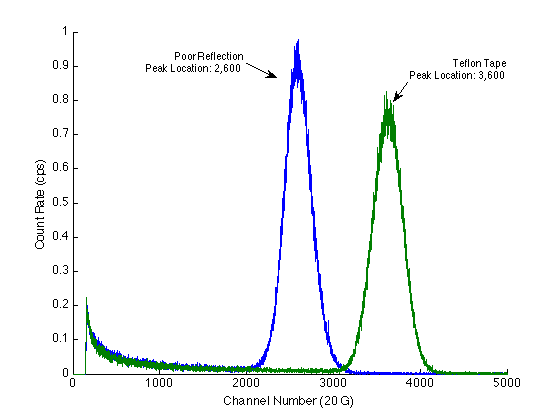
\includegraphics[width=\textwidth]{GS20_TeflonBlackTape.png}
        \end{subfigure}
        
        \begin{subfigure}[b]{\textwidth}
        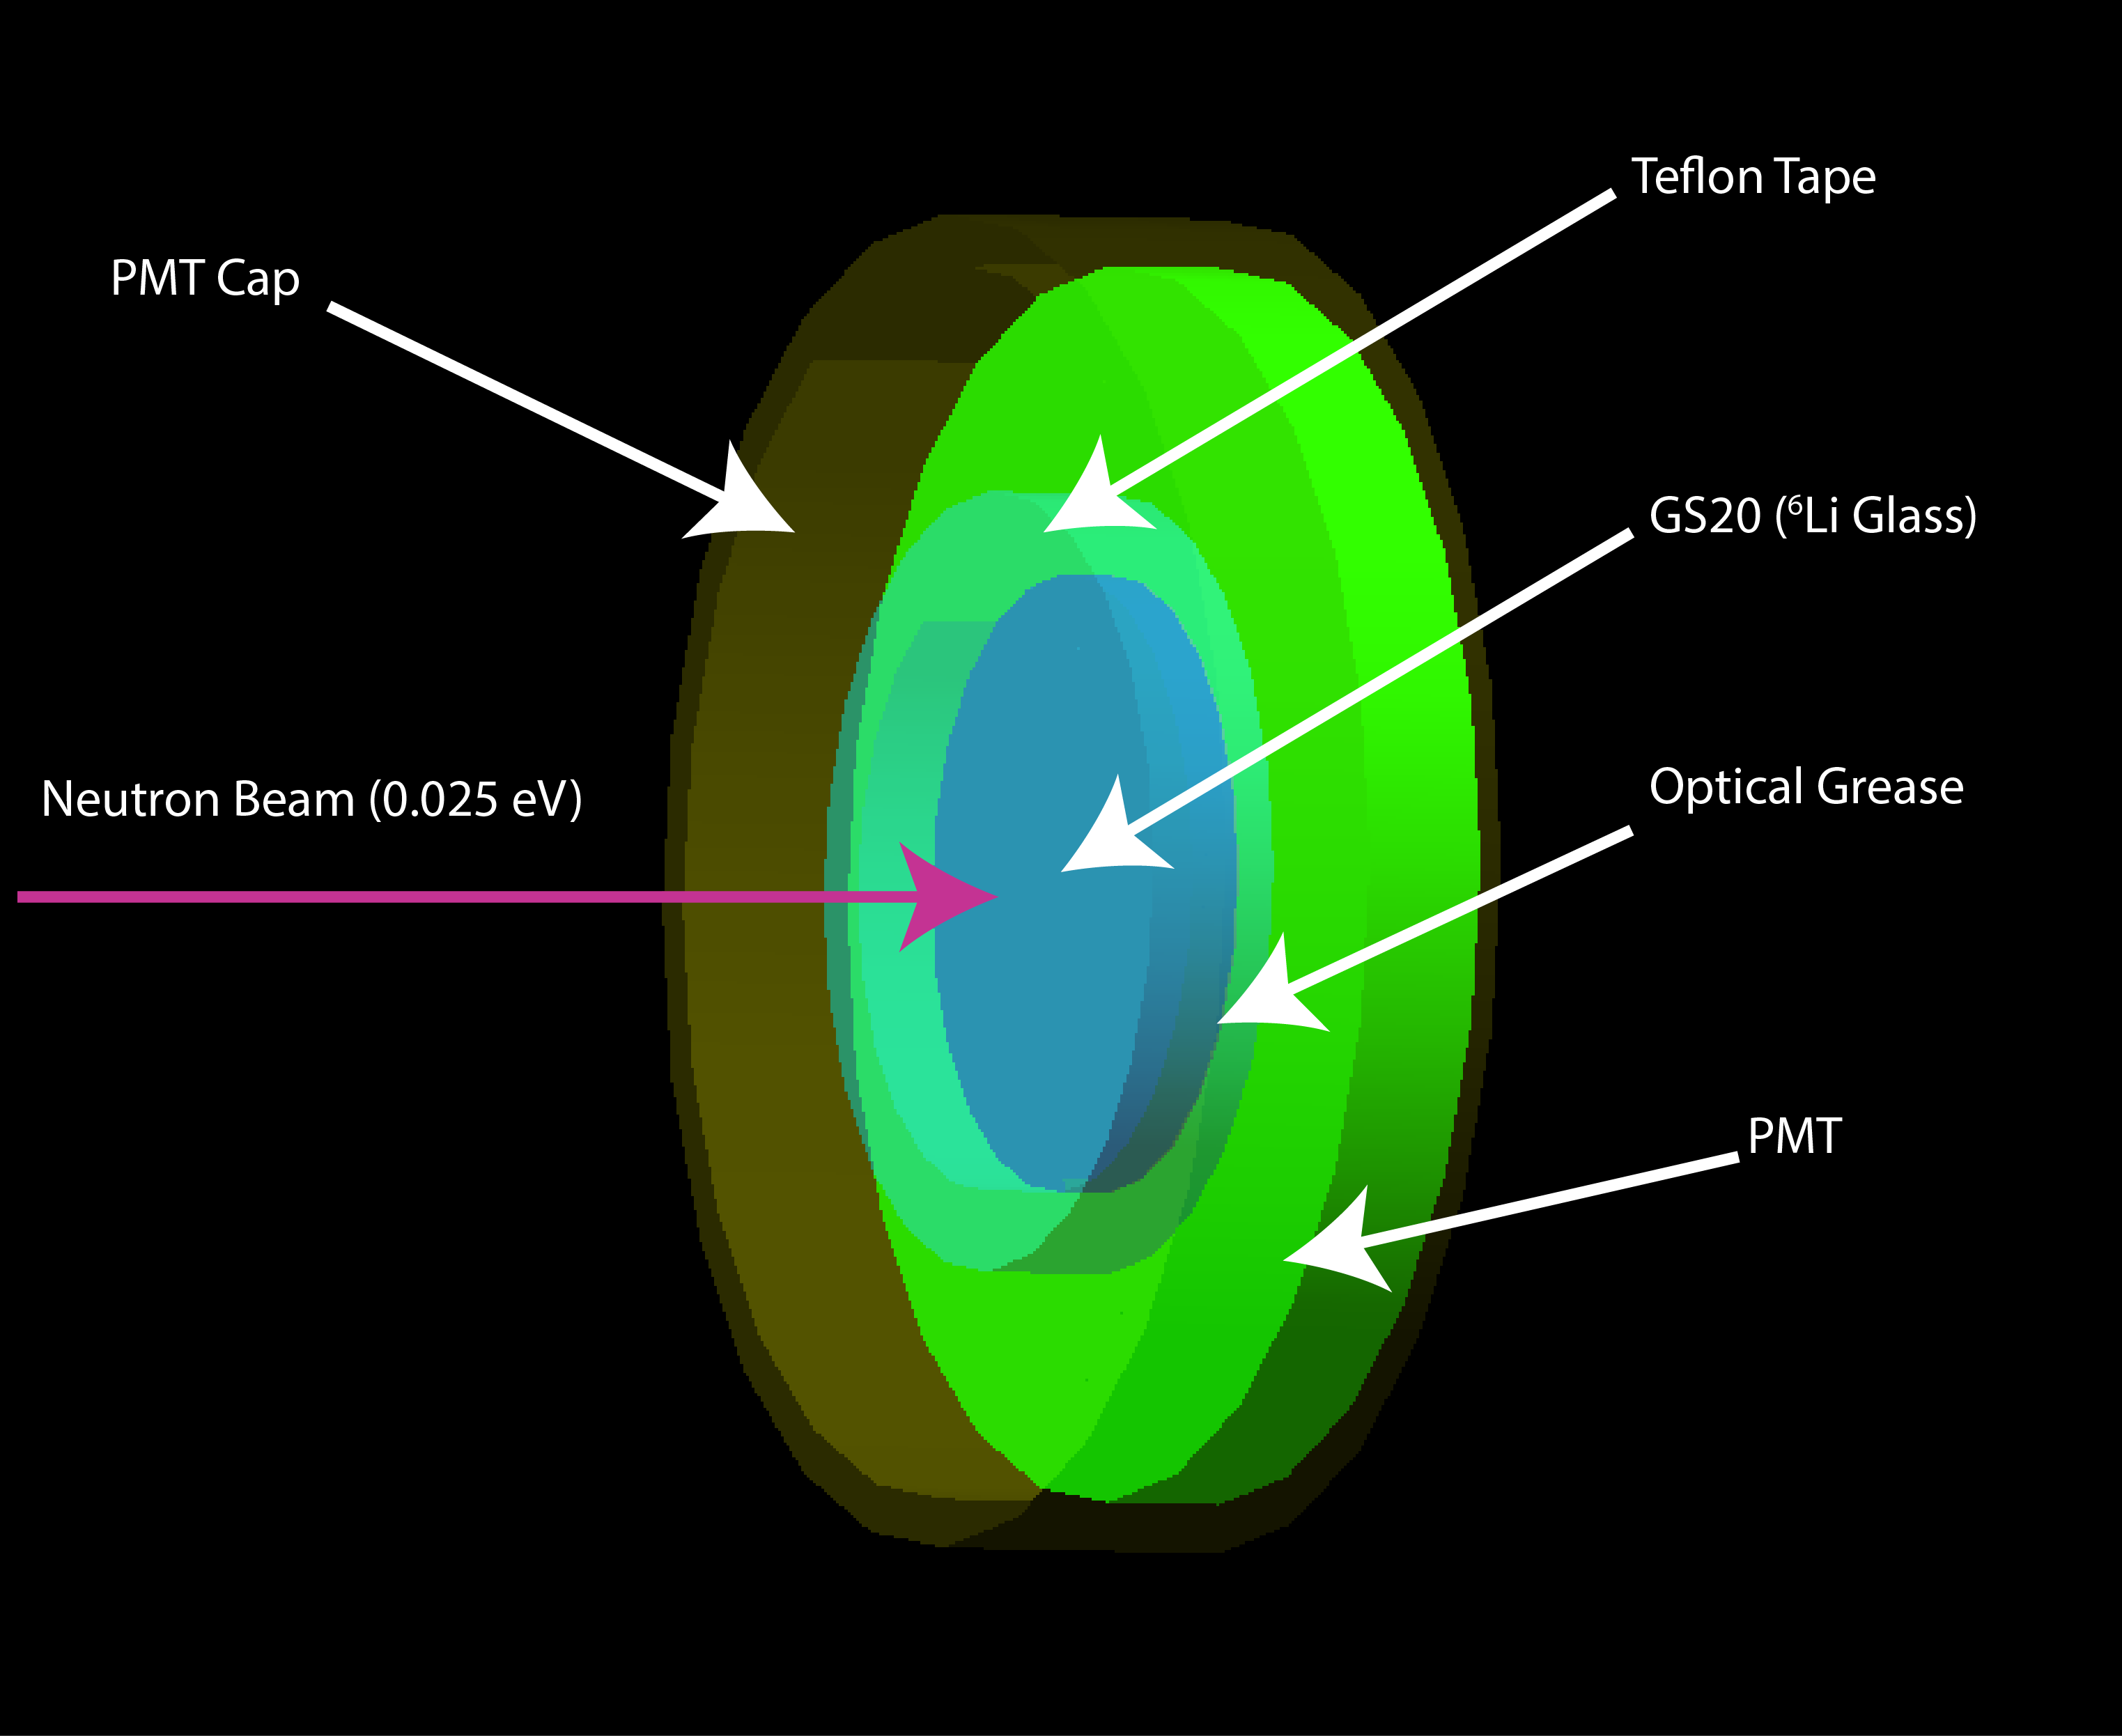
\includegraphics[width=\textwidth]{GEANT4AnnotatedGeo_GS20SimGeo.png}
        \end{subfigure}
      \end{figure}
    \end{column}
  \end{columns}
\end{frame}
%%%%%%%%%%%%%%%%%%%%%%%%%%%%%%%%%%%%%%%%%%%%%%%%%%%%%%%%%%%%%%%%%%%%%%%%%%
\begin{frame}{Small Scale Detectors}
\begin{itemize}
  \item Fabricated four 4" by 6" slab detectors
  \item Used Birks, attenuation from single film studies
  \item All values agreed within 40\%
\end{itemize}
\begin{figure}
	\centering
	\includegraphics[height=0.7\textheight]{MeasLayeredDetector_MountingLayers}
\end{figure}
\end{frame}
%%%%%%%%%%%%%%%%%%%%%%%%%%%%%%%%%%%%%%%%%%%%%%%%%%%%%%%%%%%%%%%%%%%%%%%%%%
%%%%%%%%%%%%%%%%%%%%%%%%%%%%%%%%%%%%%%%%%%%%%%%%%%%%%%%%%%%%%%%%%%%%%%%%%%
%                                                                        %
%                             RESULTS                                    %
%                                                                        %
%%%%%%%%%%%%%%%%%%%%%%%%%%%%%%%%%%%%%%%%%%%%%%%%%%%%%%%%%%%%%%%%%%%%%%%%%%
\subsection{Results}
\begin{frame}{Completed Work}
  \textbf{Neutronics, energy deposition, and light transport}
  \vspace{0.5cm}
  \begin{columns}[onlytextwidth]
    \begin{column}{0.45\textwidth}
      Geometries
      \begin{itemize}
        \item GS2O  (with and without reflector)
        \item 4 in by 6 in two layer detectors
        \item Full RPM
      \end{itemize}
    \end{column}
    \begin{column}{0.45\textwidth}
      Parameter Studies
      \begin{itemize}
        \item Light guide thickness
        \item Light guide material (WLS)
        \item Reflectivity and wrappings
      \end{itemize}
    \end{column}
  \end{columns}
\hyperlink{G4Intro}{\beamerbutton{Light Transport with GEANT4}}
\end{frame}
%%%%%%%%%%%%%%%%%%%%%%%%%%%%%%%%%%%%%%%%%%%%%%%%%%%%%%%%%%%%%%%%%%%%%%%%%%
\begin{frame}{Slab Thickness, Cladding and Light Collection Geometry}
GEANT4 simulations preformed on the slab thickness, cladding material
  \begin{figure}
    \centering
    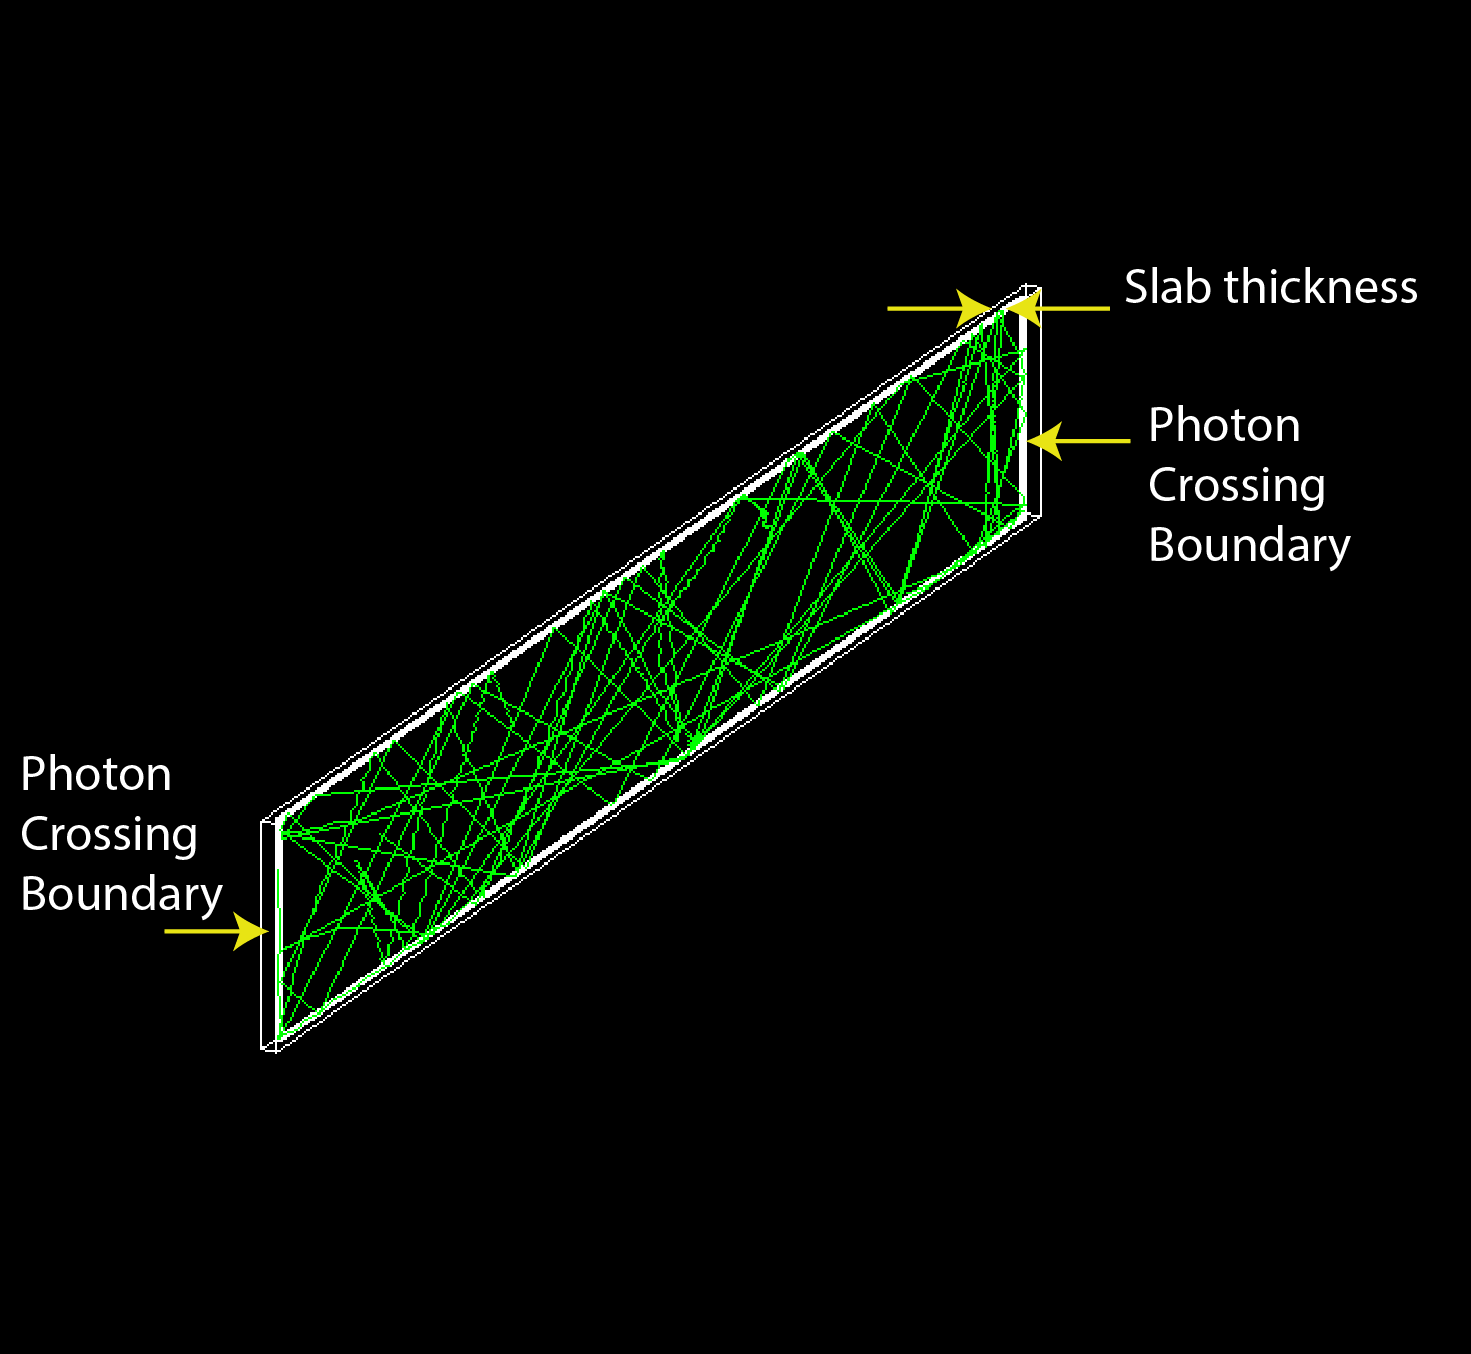
\includegraphics[height=0.7\textheight,keepaspectratio]{GEANT4AnnotatedGeo_WLSGeo}
  \end{figure}
\end{frame}
%%%%%%%%%%%%%%%%%%%%%%%%%%%%%%%%%%%%%%%%%%%%%%%%%%%%%%%%%%%%%%%%%%%%%%%%%%
\begin{frame}{Slab Thickness Effects}
Thicker slabs have better light collection
\begin{table}
	% Data for this table may be found on pg. 30 of the third lab notebook
	\small
  \begin{tabular}{c | c  c}
	\toprule
	Slab Thickness & Fraction Collected (\SI{50}{\cm}) & Fraction Collected (\SI{25}{\cm}) \\
	\midrule
	\SI{100}{\um} & 1.1\% & 1.1\% \\
	\SI{220}{\um} & 1.3\% & 1.7\% \\
	\SI{460}{\um} & 1.5\% & 1.9\% \\
	\SI{1}{\mm} & 2.2\% & 2.8\% \\
	\SI{2.2}{\mm} & 3.5\% & 4.2\% \\
	\SI{4.6}{\mm} & 5.1\% & 6.2\% \\
	\SI{1}{\cm} & 6.3\% & 7.3 \% \\
	\bottomrule
	\end{tabular}
\end{table}
\end{frame}
%%%%%%%%%%%%%%%%%%%%%%%%%%%%%%%%%%%%%%%%%%%%%%%%%%%%%%%%%%%%%%%%%%%%%%%%%%
\begin{frame}{Cladding Effects}
The material encasing the material impacts the light collection
\begin{table}
  \small
  \begin{tabular}{p{1.5cm} m{1.5cm} m{3cm} m{3cm}}
  \toprule
  & Coating & Fraction of Photons Collected & Expected Number of Photons Collected \\
  \midrule 
  \multirow{3}{*}{PS LiF} & Teflon & 4.3\% & 86\\
  				      & Air & 4.5\% & 90\\
				      & Mylar & 4.0\% & 80\\
  \midrule 
  \multirow{3}{*}{EJ-426} & Teflon & 0.46\% &736\\
  				      & Air & 0.45\% & 720\\
				      & Mylar & 0.42\% & 672 \\
 \bottomrule				 	   				  
 \end{tabular}
\end{table}
\end{frame}
%%%%%%%%%%%%%%%%%%%%%%%%%%%%%%%%%%%%%%%%%%%%%%%%%%%%%%%%%%%%%%%%%%%%%%%%%%
\begin{frame}{Simulated RPM}
  \begin{columns}[onlytextwidth]
    \begin{column}{0.45\textwidth}
		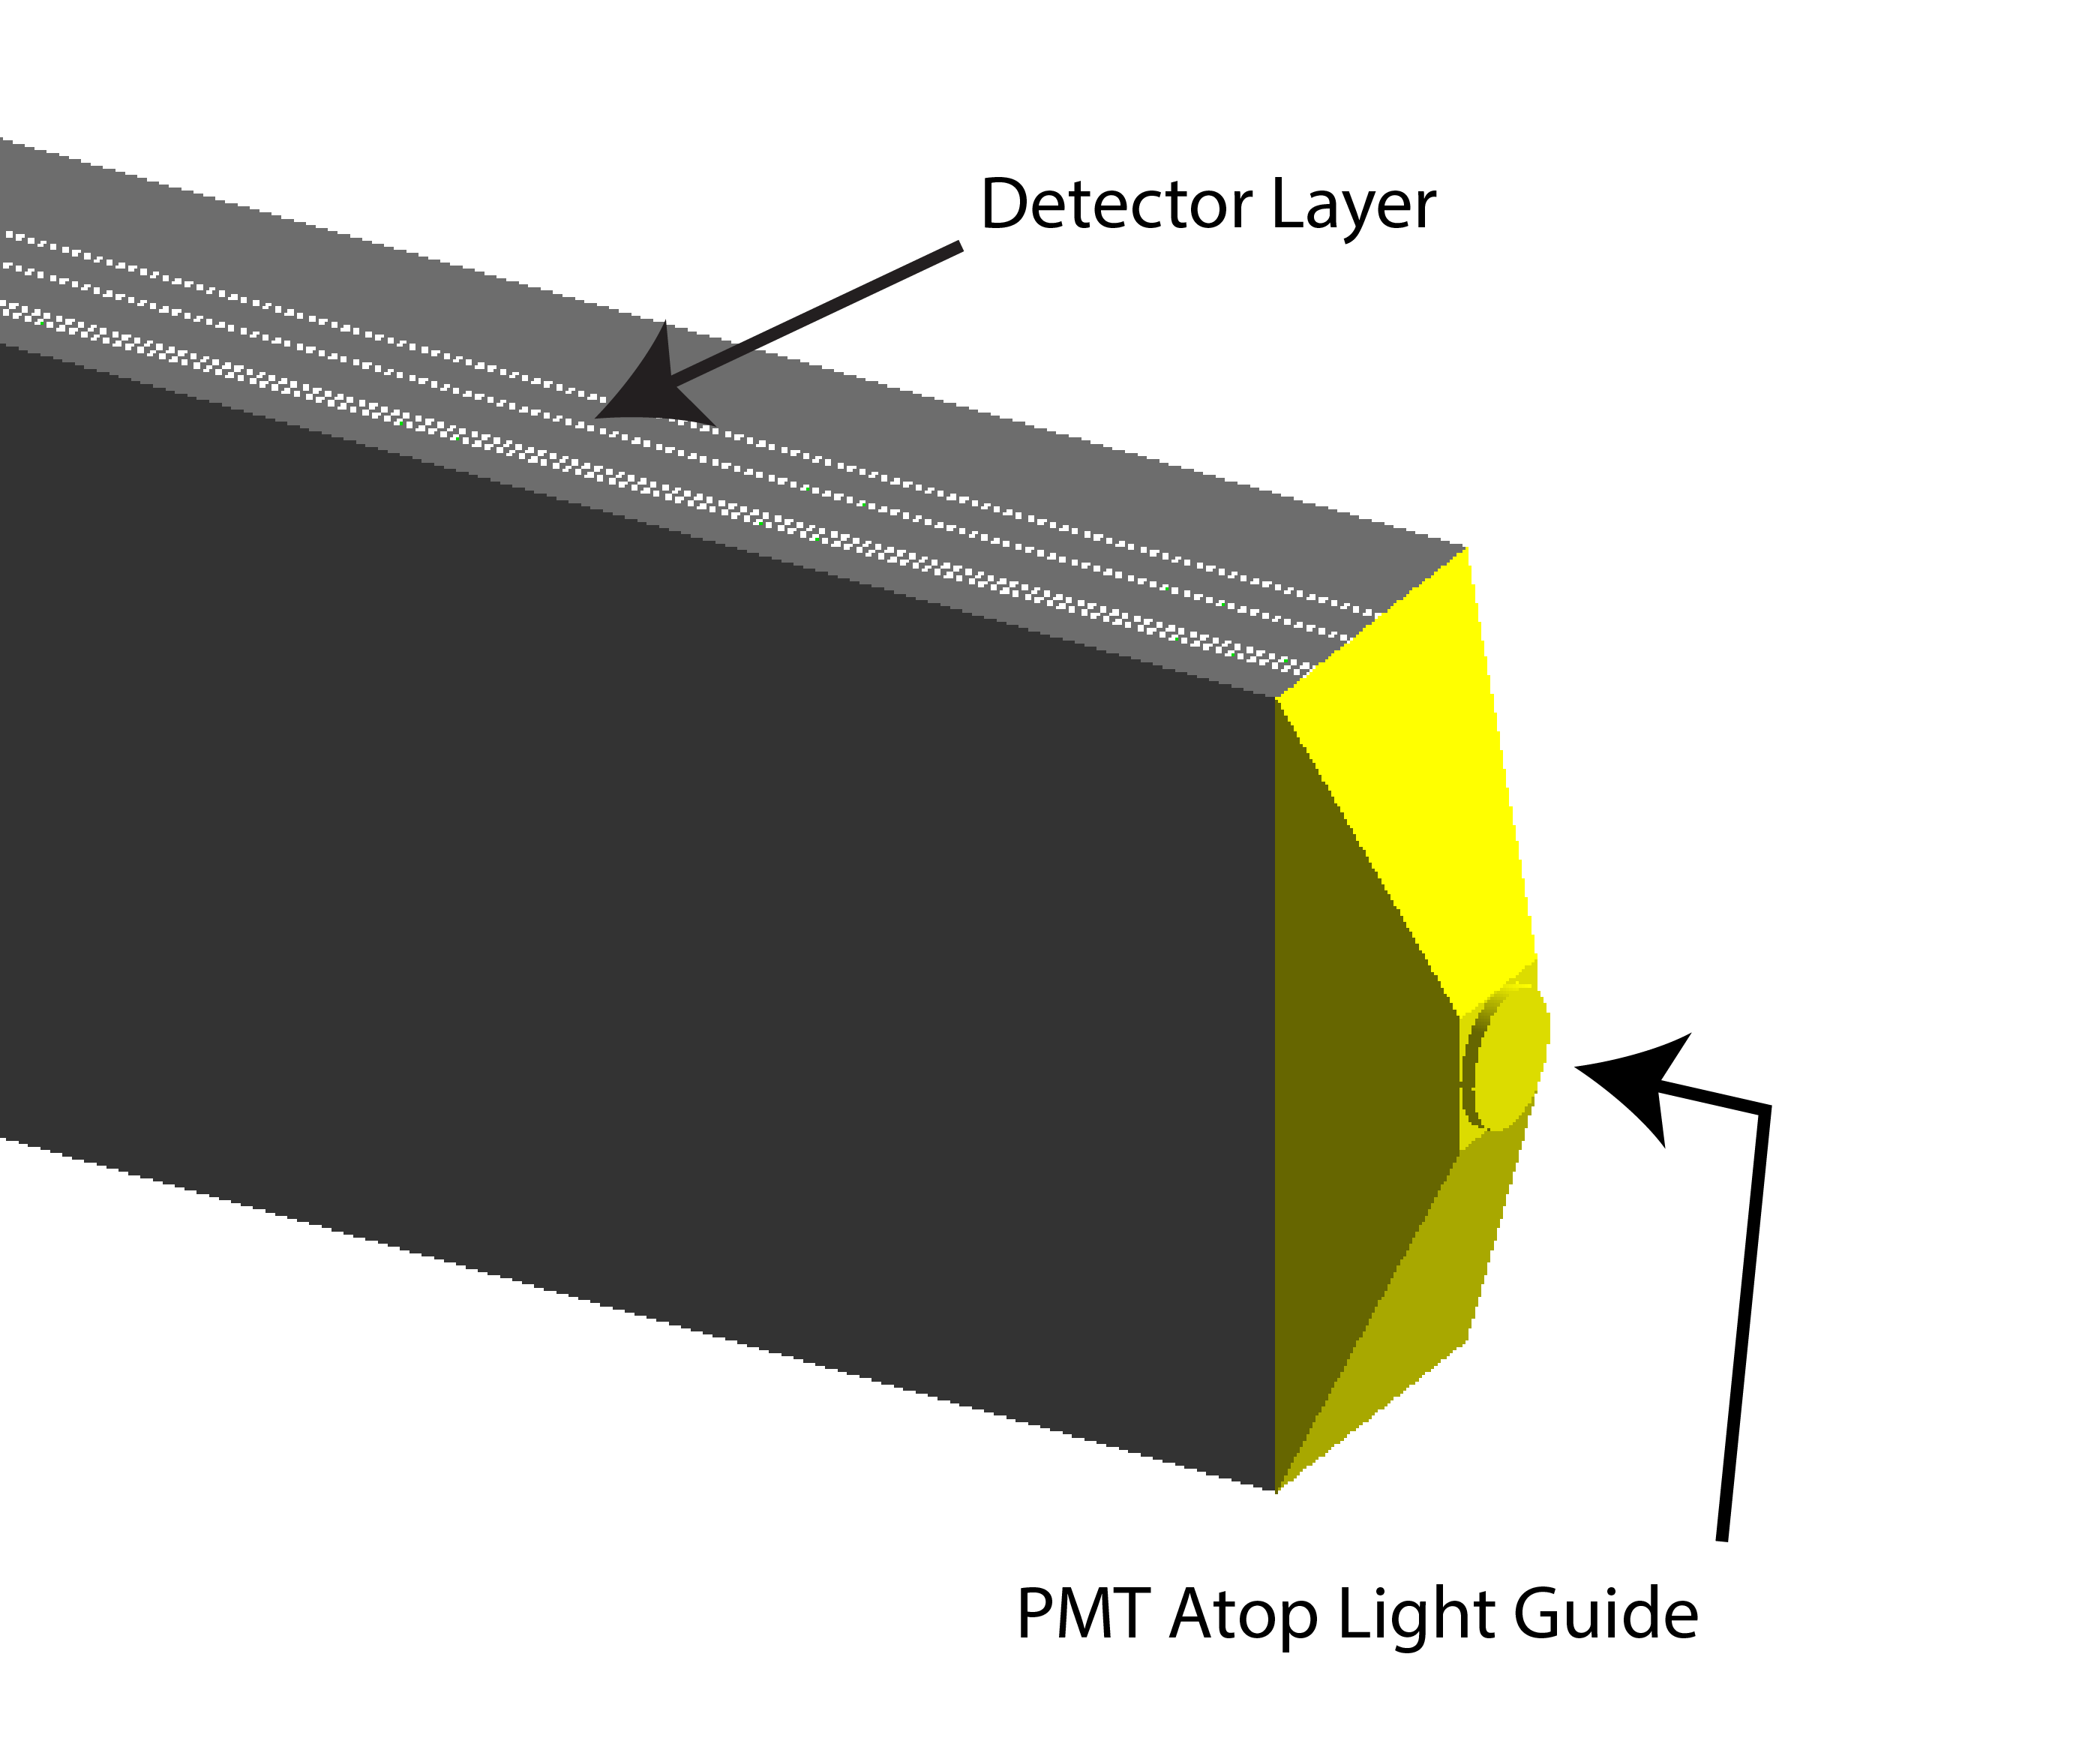
\includegraphics[width=\textwidth]{GEANT4AnnotatedGeo_RPM8SimGeoPMTEnd.png}
    \end{column}
    \begin{column}{0.45\textwidth}
		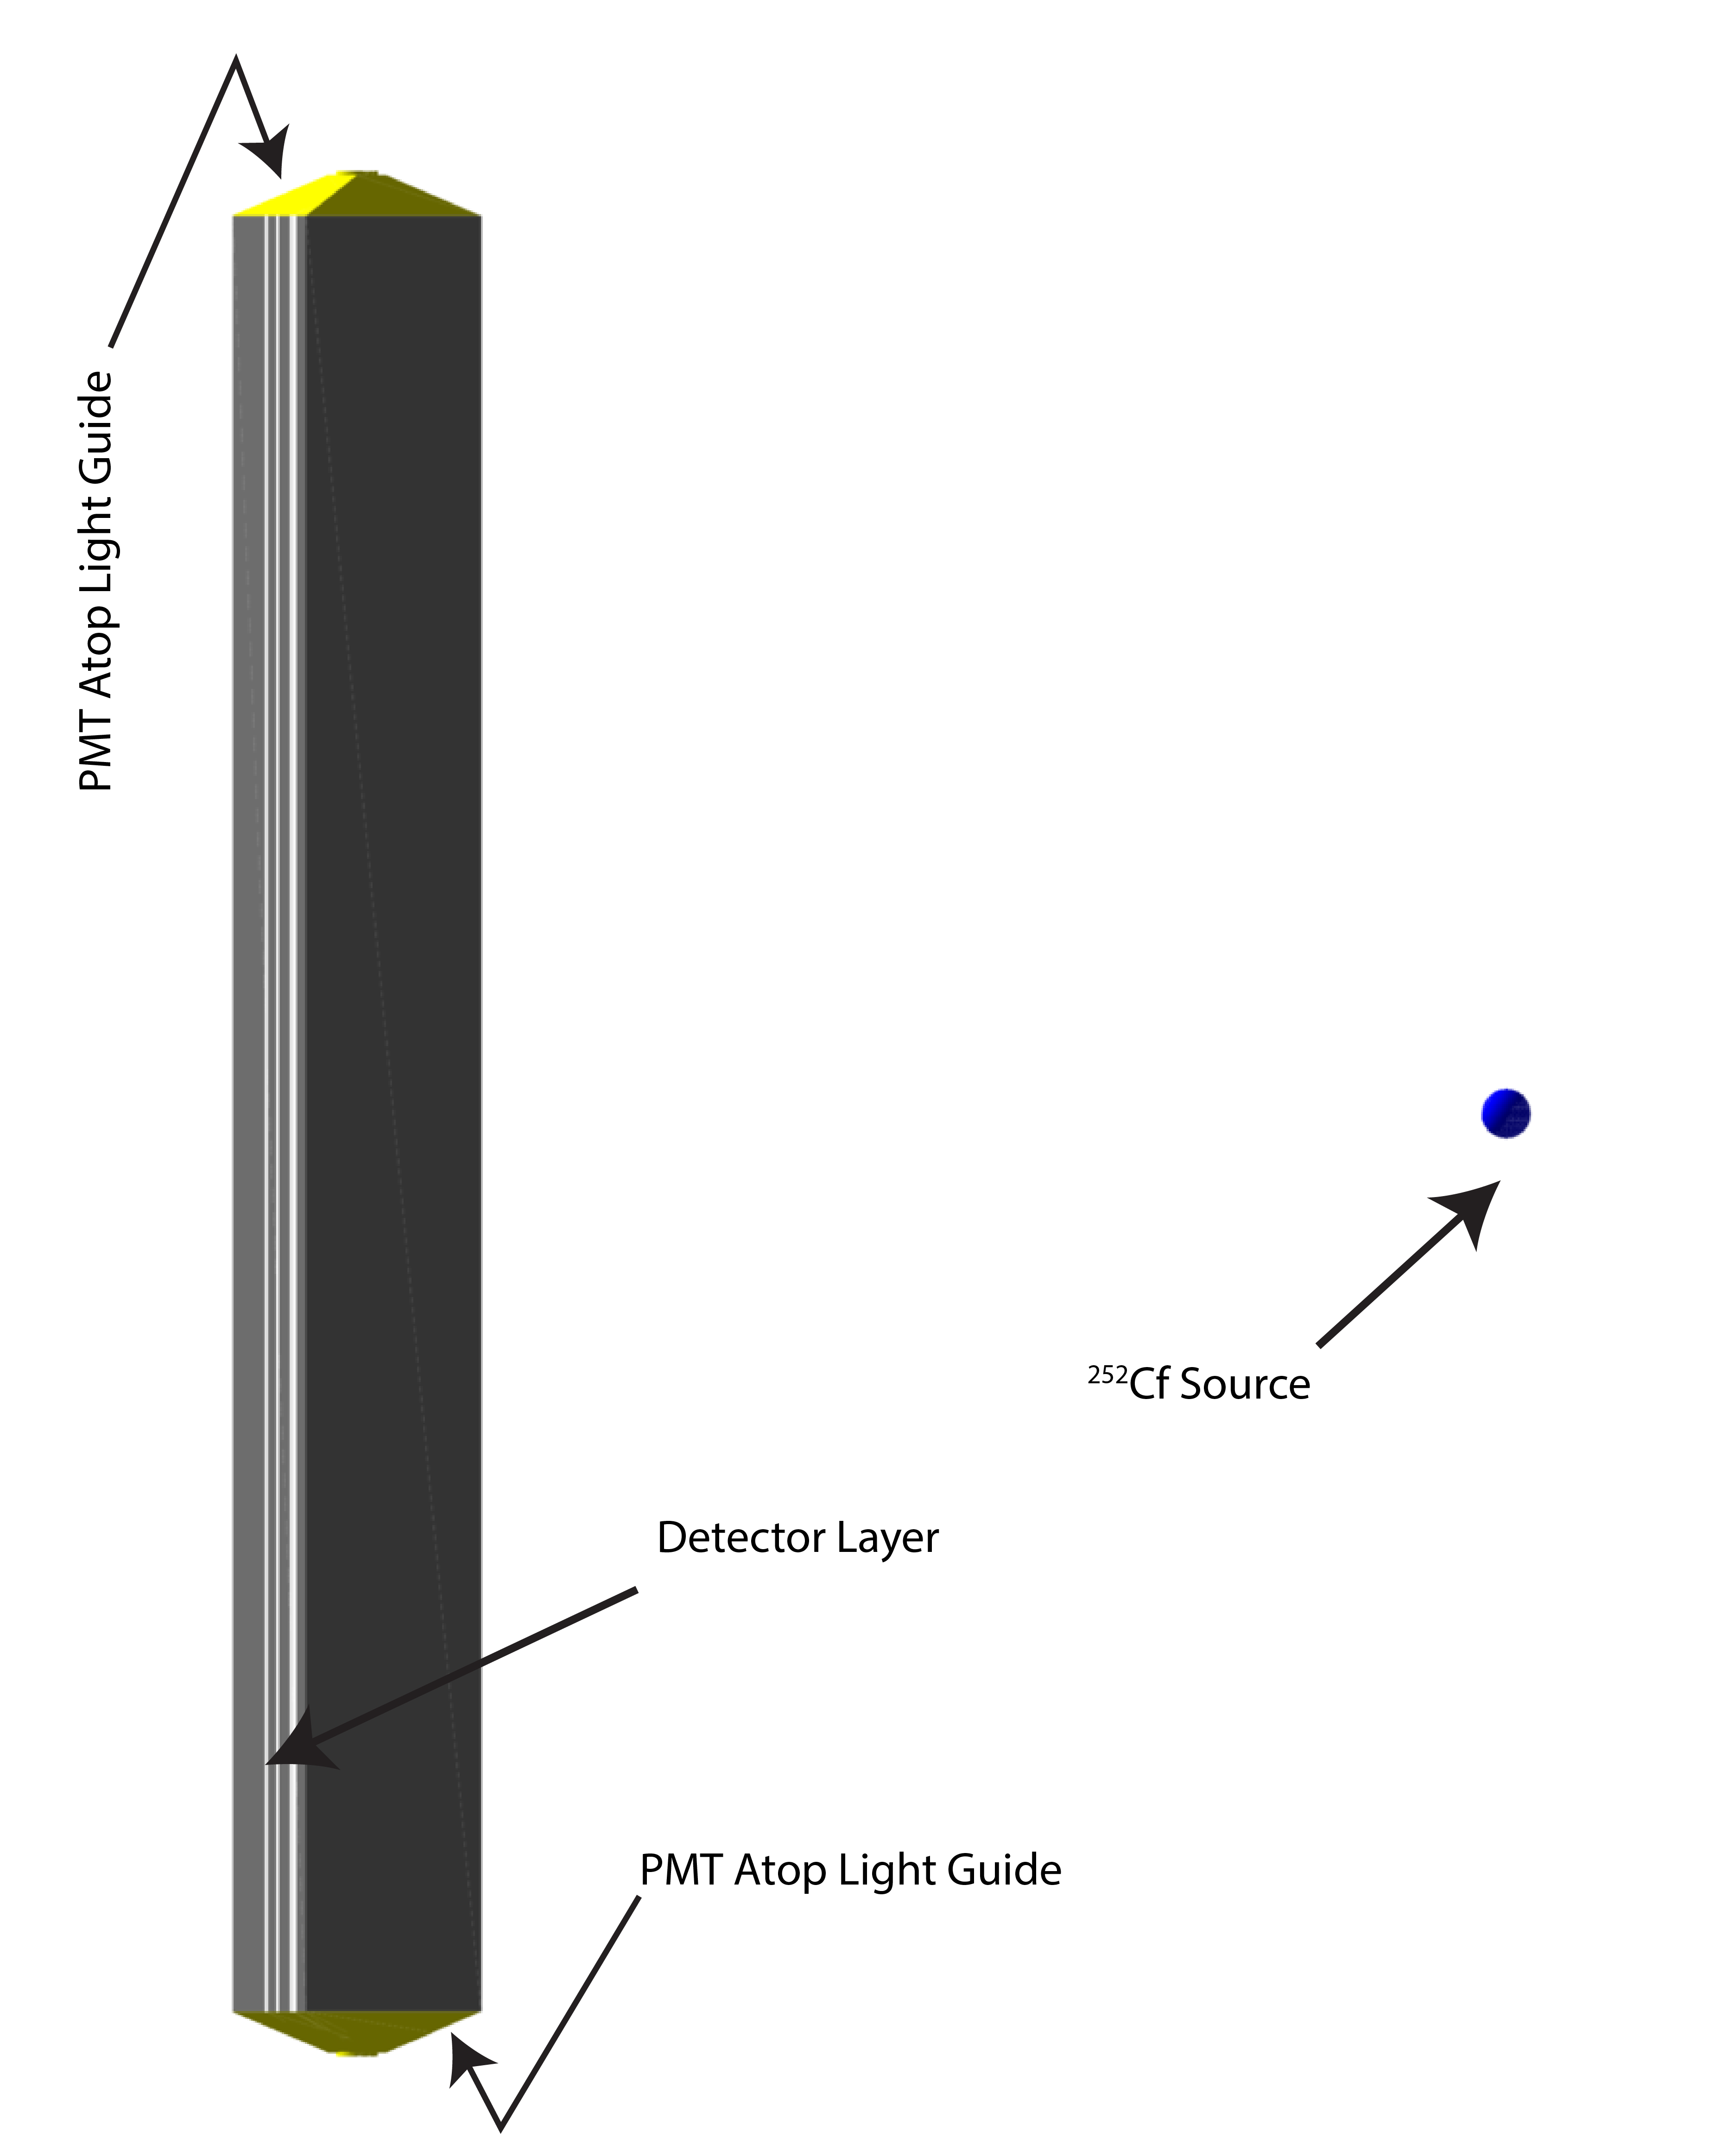
\includegraphics[width=\textwidth]{GEANT4AnnotatedGeo_RPM8SimGeo.png}
    \end{column}
  \end{columns}
\end{frame}
%%%%%%%%%%%%%%%%%%%%%%%%%%%%%%%%%%%%%%%%%%%%%%%%%%%%%%%%%%%%%%%%%%%%%%%%%%
